\label{desenvolvimento_processamento}

Nesta seção é descrito o detalhamento da solução do módulo de interface/processamento, resultante das duas primeiras fases, 
e o seu projeto e construção, resultante da Fase 03. Além disso, a visão da solução e da arquitetura podem ser vistas nos Apêndices
\ref{documento_visao} e \ref{documento_arquitetura}.

\subsection{Detalhamento da Solução} \label{software:detalhamento_solucao}
Esta subseção apresenta a visão da solução da parte de processamento e interface referentes a Software, e
integração com a frente de Eletro-eletrônica. A intenção desta frente é apresentar a visão da arquitetura do sistema,
bem como será o fluxo de dados entre usuário até chegar ao sistema. A intenção é transmitir as decisões significativas do 
ponto de vista da arquitetura de baixo e alto nível que foram tomadas de acordo com as necessidades do sistema.

\subsubsection*{\textbf{Escopo}}

A arquitetura que foi idealizada fundamenta a base para a construção do produto, expressando como o sistema deverá se 
comportar em suas interações, bem como o nível de abrangência da aplicação em quesitos de limitação e qualidade.

O escopo deste projeto vai de encontro em cobrir os aspectos de comunicação entre usuário e sistema, bem como o tratamento
dos dados embarcados. Para isso, este será apresentado o dimensionamento do sistema, tanto em alto nível, com relação à aplicação 
web, quanto em baixo nível, referente a rotina de comunicação entre Raspberry PI e Arduino e a rotina de processamento de dados.

\subsubsection*{\textbf{Representação da Arquitetura}}

A arquitetura da aplicação utiliza de padrões que organizam e aperfeiçoam o desenvolvimento dentro do paradigma de Orientação a 
Objetos e adicionalmente, a persistência e o consumo de dados.

Quanto à camada de alto nível, para o corrente projeto da bancada de vibrações, optou-se por desenvolver uma aplicação web para que 
o usuário possa fornecer inputs de controle para operação da bancada e também, visualizar os resultados do ensaio realizado.

É válido ressaltar que para fins de boa performance da aplicação web, foram consideradas abordagens para o projeto de aplicativos 
da Web fracamente acoplados. Nesse cenário, o estilo REST (Representational State Transfer - Transferência de Estado Representacional)
foi adotado.

Roy Fielding, um dos idealizadores do estilo REST,  afirma que o estilo REST enfatiza a escalabilidade das interações entre 
componentes e componentes intermediários para reduzir a latência da interação.

De uma forma geral, vale notar que tudo na Web (páginas, imagens, entre outros) são a essência de um recurso \footnote{http://www.ibm.com/developerworks/br/library/j-rest/}.
O fato de o REST  possuir a  característica de contar com recursos nomeados em vez de mensagens facilita o fraco acoplamento 
no design da aplicação.

Logo abaixo, é possível contemplar uma figura esquemática da arquitetura geral do sistema.

\begin{figure}[!ht]
\centering
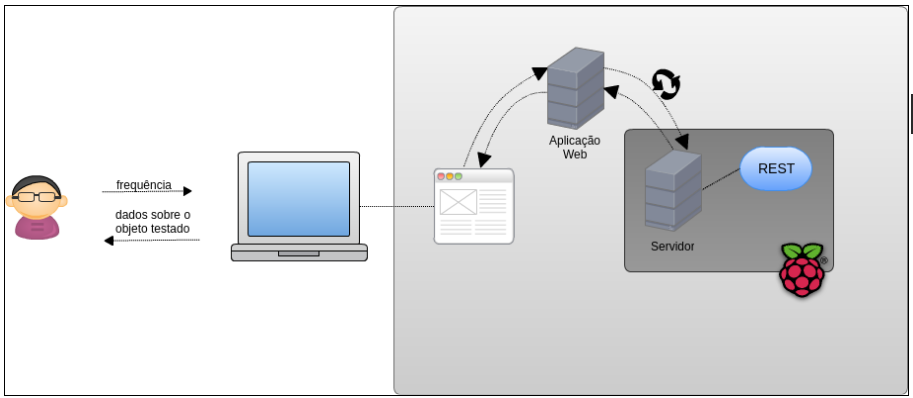
\includegraphics[scale=0.5]{figuras/arquitetura_sistema.png}
\caption{Esquema geral da arquitetura do sistema. Fonte: Autores}
\label{fig:arquitetura_sistema}
\end{figure}

Para a realização dos testes na bancada, o usuário poderá determinar a frequência de vibração e o tempo de funcionamento da 
bancada por meio da interação com uma aplicação web. Durante e após a execução dos testes, o usuário poderá visualizar os dados
coletados pelos sensores.

A aplicação web fará requisições, através de uma rotina, para um servidor que provê serviços REST. Este servidor será disponibilizado
por uma Raspberry Pi. É valido ressaltar que a comunicação entre aplicação web e o Raspberry PI funcione é necessário que o mesmo 
esteja com acesso a internet para que ele possa receber e enviar as requisições para a aplicação web.

Adicionalmente, os serviços REST consultarão os dados coletados e persistidos em uma base de dados SQLite , que também será hospedado
na Raspberry Pi.

Para a camada de baixo nível será desenvolvido uma rotina responsável por enviar, receber dados entre Arduino e Raspberry PI, bem 
como disponibilizar os dados recebidos na forma de arquivos que serão utilizados pela aplicação para que o usuário consiga ver os 
resultados das ações que foram aplicadas no sistema. Toda essa transmissão de dados será feita com a interface UART \footnote{http://www.raspberry-projects.com/pi/programming-in-c/uart-serial-port/using-the-uart}
(Universal Asynchronous Receiver Transmitter - Transmissor Receptor Assíncrono Universal), via serialização de dados.

Os dados de resultados que chegarem do Arduino para a Raspberry PI, serão tratados pela rotina de comunicação de forma a 
disponibilizar esses dados brutos em arquivos. Estes arquivos serão lidos por uma rotina que terá como objetivo realizar o 
processamento dos dados e logo em seguida a realização do parser (leitura dos dados nos arquivos e a gravação deles no banco 
de dados embarcado) desses dados no banco de dados local.

\begin{figure}[!ht]
\centering
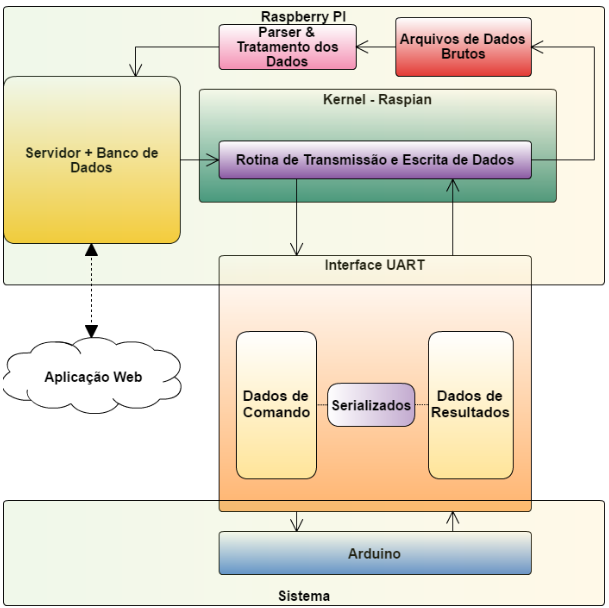
\includegraphics[scale=0.5]{figuras/sistema.png}
\caption{Camada baixo nível do sistema, responsável pela comunicação entre a aplicação web e o sistema da bancada de vibração}
\label{fig:sistema}
\end{figure}

Por fim, vale destacar que a rotina é o meio de integração entre Software e Eletrônica o qual teremos uma comunicação
de baixo nível pela porta serial e os resultados obtidos entregues na forma de arquivos, ou seja, separando a comunicação 
entre Hardware e a aplicação. Serão utilizados rotinas para tratamento dos dados de acordo com a necessidade do usuário em 
visualizar os dados de resultados derivados.

\subsubsection*{\textbf{Restrições Arquiteturais}}
Com o objetivo de se criar um sistema confiável, estabeleceu-se que deverá ser feita uma avaliação dos componentes mais críticos 
e deverão ser elaborados testes unitários para assegurar o bom funcionamento destes módulos.

Adicionalmente, dentre as opções de linguagens de programação disponíveis para desenvolvimento de aplicações web, e do parser e 
tratamento dos dados brutos, optou-se pela linguagem Python e para a camada de baixo nível será utilizado a linguagem C para o 
desenvolvimento  das rotinas de comunicação entre Raspberry PI e Arduino. O desenvolvimento da aplicação web e dos serviços REST 
será feito com o auxílio de recursos providos pelo framework Django \footnotemark, que oferece uma alta produtividade no 
desenvolvimento.
\footnotetext{https://www.djangoproject.com/}

A linguagem de programação Python possui uma excelente performance, especialmente considerando que o hardware a ser utilizado 
para disponibilizar o servidor REST possui recursos de processamento bem limitados. Além disso, a linguagem de programação Python 
possui uma alta produtividade associada.

Outro aspecto vantajoso da linguagem é vasta disponibilidade de bibliotecas para tratamento de informações, especialmente cálculos
matemáticos, que serão amplamente utilizados no sistema para uso integrado com a bancada de vibrações.
\newpage
\subsubsection*{\textbf{Requisitos Levantados}}
A partir do escopo definido no projeto foram elicitados alguns requisitos de forma macro, estes podem ser vistos na 
Figura \ref{backlog_produto} que representa os \textit{Backlogs} do Produto para as duas aplicações.

\begin{figure}[H]
\centering
\label{backlog_produto}
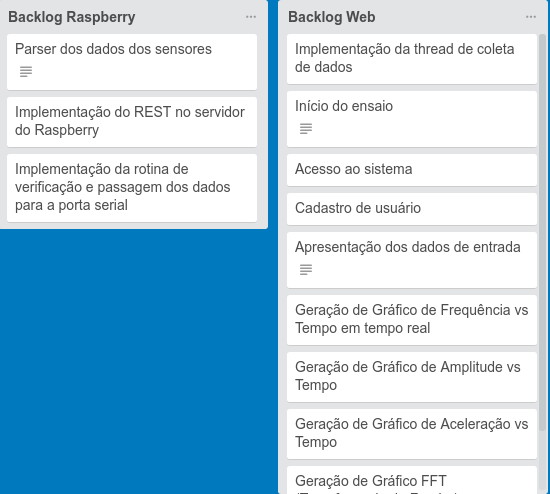
\includegraphics[keepaspectratio=true,scale=0.55]	{figuras/backlog_produto.png}
\caption{\textit{Backlogs} das aplicações do projeto}
\end{figure}

\subsubsection*{\textbf{Protótipo da Solução Web}}

Com o intuito de visualizar a solução Web foi desenhado um protótipo de alta fidelidade da aplicação Web. 
As telas podem ser vistas no \href{https://drive.google.com/file/d/0B5InkGKx6O-MR1B3eVYzZFpjQ3c/view?usp=sharing}{Relatório 1}. 

\subsection{Projeto e Construção}

Nesta subseção é apresentado o projeto e construção do sistema proposto na Subseção \ref{software:detalhamento_solucao}, bem
como as mudanças realizadas no que foi proposto.

\subsubsection*{\textbf{Mudanças - Rotinas de Comunicação}}

A camada de software na aplicação Web foi desenvolvida em \textit{Python}, bem como a camada de servidor de comunicação com a aplicação na 
\textit{Raspberry}. Como foi relatado, os membros do grupo naquele momento haviam chegado ao consenso de utilizar a linguagem C para integrar 
com \textit{Python}, que seria utilizado nas rotinas de comunicação entre \textit{Raspberry} e os microcontroladores da baixa aplicação.

Durante o desenvolvimento das rotinas de comunicação, foi-se percebendo que não havia necessidade de que o mesmo fosse desenvolvida 
usando tal linguagem, considerando que a linguagem C é uma linguagem de baixo nível normalmente utilizada para ter um maior controle sobre o 
hardware, que não é o caso. Levando em consideração este fato, foi levantada a hipótese de utilização do módulo de comunicação serial que o próprio 
\textit{Python} oferece, e para isso foi realizado uma lista de prós e contras a cerca da linguagem no desenvolvimento das rotinas de comunicação.

Utilizando a linguagem C para o desenvolvimento das rotinas de comunicação possui as seguintes vantagens:

\begin{itemize}
    \item A linguagem C é uma linguagem de baixo nível, ou seja, oferece um maior controle do hardware, e te da possibilidade de manipulações com \textit{bytes} em uma maior flexibilidade do que as outras linguagens com exceção da linguagem \textit{ASSEMBLY}.
    \item Com a linguagem C é possível desenvolver o sistema de forma a se proteger contra falhas críticas, impedindo de repassar erros de baixo nível para a camada de alto nível.
    \item A linguagem C realiza processamentos mais velozes em comparação com as outras linguagens como \textit{Python}, dentre outras, se tornando uma excelente ferramenta para manipulação de \textit{bytes}.
\end{itemize}

Desvantagens da utilização da linguagem C para o desenvolvimento das rotinas de comunicação:

\begin{itemize}
    \item Por ser uma linguagem de baixo nível com uma alta tipagem, o trabalho de desenvolver uma rotina de comunicação serial usando recursos da camada de hardware se tornam bastante complexos.
    \item Na arquitetura proposta no primeiro ponto de controle, as rotinas de escrita e leitura de dados funcionariam da seguinte maneira, a escrita iria ler um arquivo, em seguida iria apagá-lo enviaria este dado para o sistema de controle, e no sistema de leitura, seria aberta a porta seria para leitura dos \textit{bytes}, que seriam decodificados e transcritos num arquivo para serem lidos por uma rotina \textit{Python} para escrever no banco de dados. Ou seja, a integração possui uma alta complexidade.
    \item Apesar da linguagem C ser mais rápida que \textit{Python}, não existe necessidade das rotinas serem desenvolvidas em tal linguagem, pois a diferença de velocidade de escrita e leitura para comunicação serial é bem mínima levando em consideração ao que \textit{Python} também faz.
\end{itemize}

Vantagens em utilizar \textit{Python} para o desenvolvimento das rotinas de comunicação:

\begin{itemize}
    \item Python possui uma baixa tipagem.
    \item Possui uma biblioteca de comunicação serial que realiza a abstração do jeito que o desenvolvedor quiser (seja controlar em baixo nível, ou em alto nível com uma abstração do controle).
    \item Fácil integração com \textit{RESTful} do \textit{Django} que é realizado em \textit{Python}.
    \item Elimina necessidade de escrever e ler em arquivos, pois os métodos podem ser carregados pelo \textit{REST} diretamente, assim o \textit{REST} terá o controle total da comunicação.
    \item Não existe necessidade de manipular leitura e escrita de bytes, devida a abstração da biblioteca.
    \item \textit{Python} é uma linguagem melhor para manipulação de dados, e permitirá a escrita dos dados recebidos diretamente no banco de dados do servidor da \textit{Raspberry}, que a aplicação irá ler.
\end{itemize}

Desvantagens da linguagem \textit{Python} para o desenvolvimento das rotinas de comunicação:

\begin{itemize}
    \item \textit{Python} é uma linguagem interpretada e mais lenta em comparação a linguagem C.
    \item Não fornece um controle maior em comparação as linguagens de baixo nível.
\end{itemize}

Com a nova mudança então, a única linguagem de programação que está sendo utilizada neste projeto é a linguagem \textit{Python}, e em virtude 
desta mudança, a arquitetura mudou um pouco agora sendo nesse novo estilo.

\begin{figure}[H]
\centering
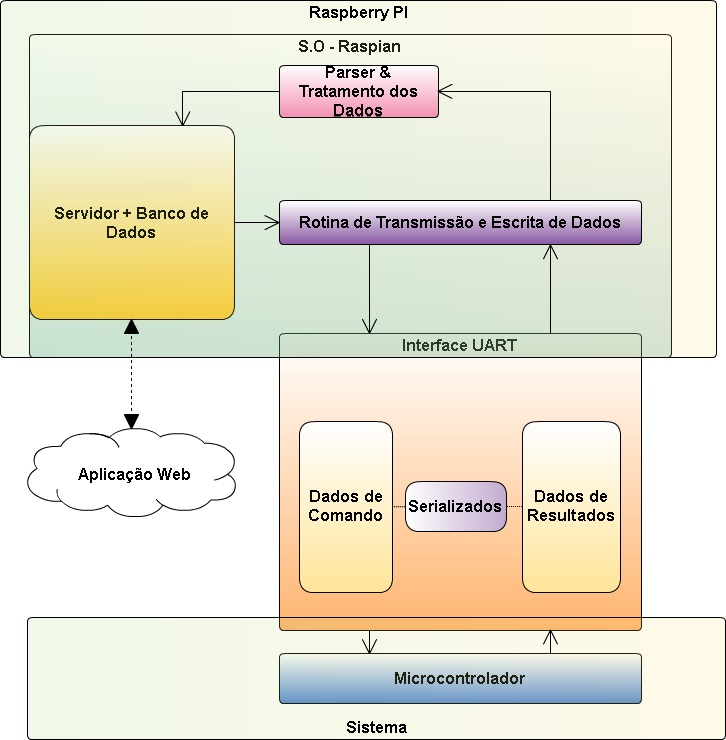
\includegraphics[keepaspectratio=true,scale=0.7]{figuras/nova_arquitetura.png}
\label{fig:nova_arquitetura}
\caption{Nova arquitetura com a mudança da linguagem implementada - Fonte: Autor}
\end{figure}

\subsubsection*{\textbf{Protocolo de Comunicação}}

As rotinas de comunicação são as pontes pela qual a frente de software irá se comunicar com a frente de eletroeletrônica e com o resto do sistema. 
Para que a comunicação seja estabelecida, foi necessário estabelecer um padrão de comunicação de acordo com ambas as frentes, de forma que a comunicação 
ocorra com sucesso e sem surpresas. Foi definido então um protocolo de comunicação ao qual deverá ser respeitado entre a frente de software e eletrônica, 
durante a transmissão de dados via serial.

Com a mudança da arquitetura, acabou facilitando a integração das rotinas de comunicação e escrita com parser e com o servidor e nos permitiu formalizar 
um protocolo bem simples para comunicação entre sistema de controle e sistema da aplicação.

Protocolo de comunicação é descrito da seguinte forma: Ele é dividido em duas partes, em protocolo de controle e protocolo resposta.

\begin{itemize}
    \item Protocolo de Controle
    \begin{itemize}
        \item É definido por \textit{flags} que permitirão que o sistema realize ações pré-definidas.
    \end{itemize}
    \item Protocolo de Resposta
    \begin{itemize}
        \item É definido a \textit{STRING} de resposta que o sistema de controle enviará para a camada de alto nível no caso a \textit{Raspberry} via 
        comunicação serial.
    \end{itemize}
\end{itemize}

\begin{figure}[H]
\centering
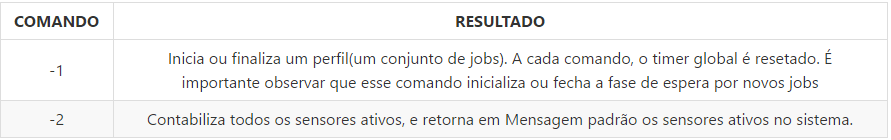
\includegraphics[keepaspectratio=true,scale=0.7]{figuras/protocolo_controle.png}
\label{fig:protocolo_controle}
\caption{Protocolo de Controle com \textit{flags} já definidas - Fonte: Autor}
\end{figure}

\begin{figure}[H]
\centering
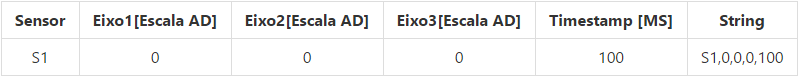
\includegraphics[keepaspectratio=true,scale=0.8]{figuras/protocolo_string.png}
\label{fig:protocolo_string}
\caption{Protocolo de Resposta e o formato da String que chegará ao sistema - Fonte: Autor}
\end{figure}

Com esse padrão definido, o usuário definirá um determinado número de \textit{jobs} (cada \textit{job} representa uma frequência com uma duração de tempo, 
e um conjunto de \textit{jobs} define um ensaio) que serão executados ao longo do ensaio. Ao executar o ensaio, o resultado dos sensores irão ser 
repassados na escala entre 0 a 1024 em AD (\textit{Analogic Digital}), sendo 0AD igual a 0G e 1024AD igual a 16G, ou seja, com uma regra de três simples,
determinará as acelerações dos pontos de acordo com a frequência estabelecida e, por fim, esses dados passarão pelo processamento, para serem salvos no 
banco de dados da \textit{Raspberry}.

Um dos objetivos ao obter a \textit{timestamp} a qual foi obtido o resultado pelo sensor, será para realizar o mapeamento dos \textit{jobs} de acordo 
com o ensaio, para ordenar e saber quais dados pertencem a quais \textit{jobs}.

Na imagem \ref{fig:diagrama_sequencia_pc2}, mostra um diagrama de sequência entre usuário, a aplicação web, o servidor da \textit{raspberry}, sobre 
como é tratado o \textit{input} e o \textit{output} do sistema como um todo entre as frentes da software e eletrônica.

\begin{figure}[H]
\centering
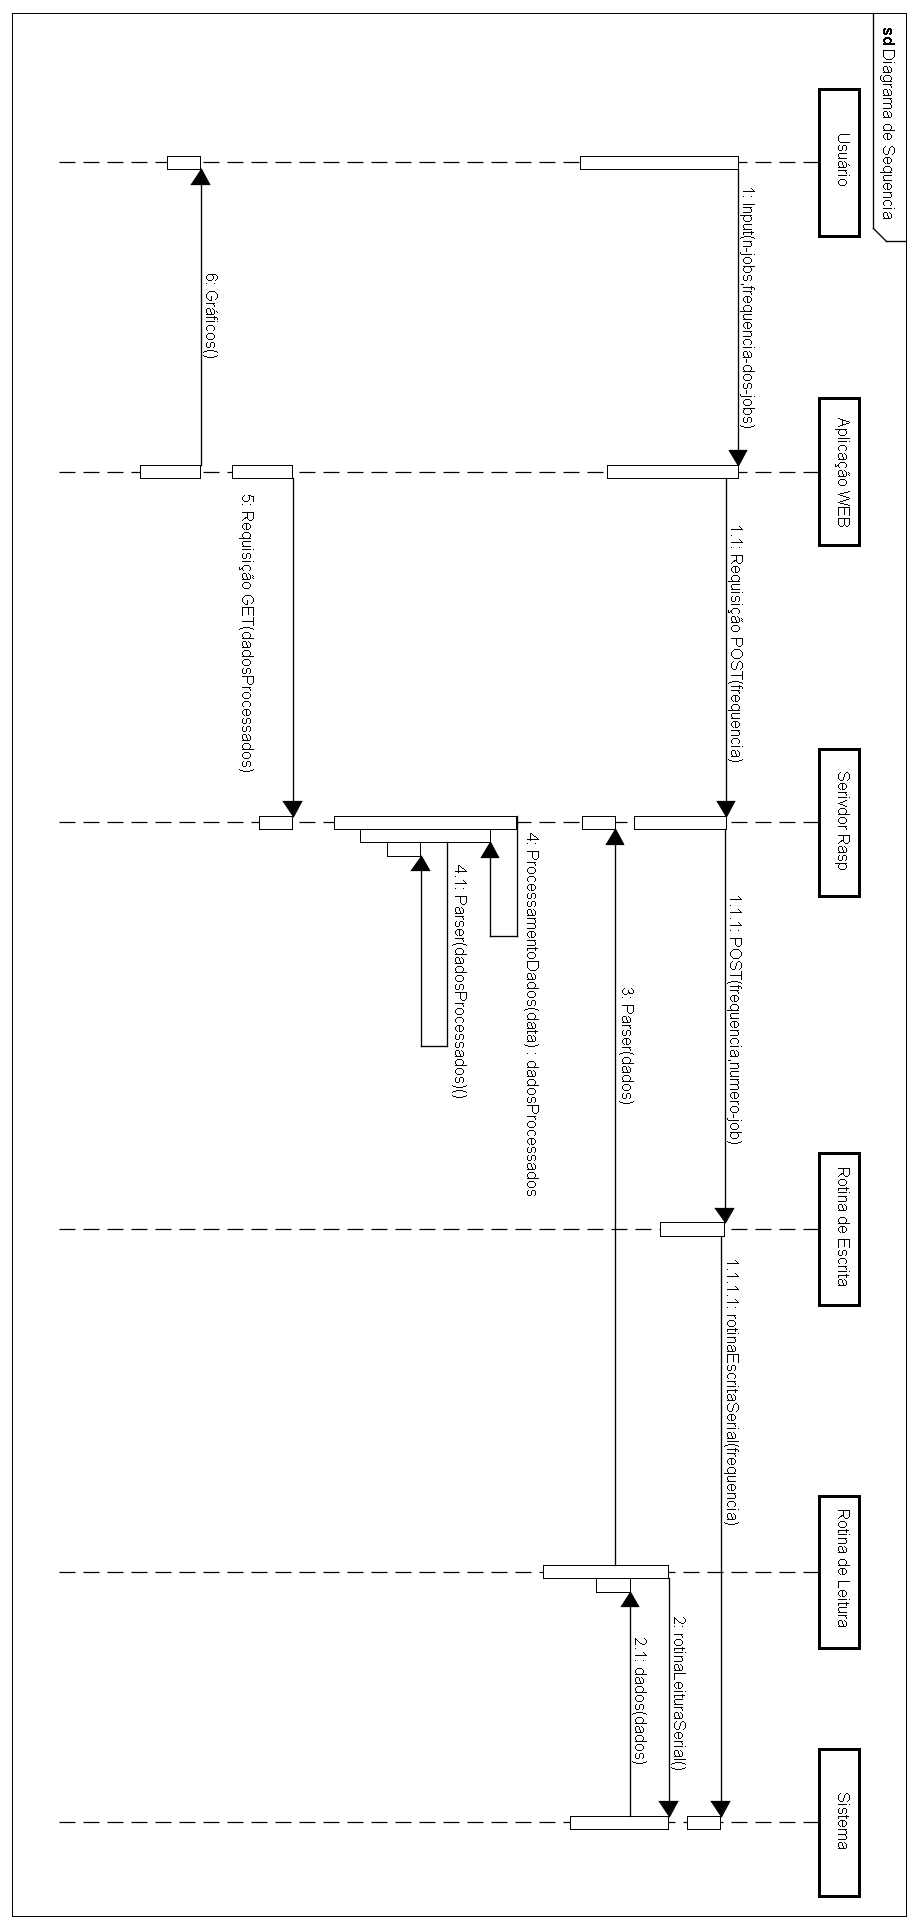
\includegraphics[keepaspectratio=true,scale=0.5]{figuras/diagrama_sequencia_pc2.png}
\label{fig:diagrama_sequencia_pc2}
\caption{Diagrama de sequência - Fonte: Autor}
\end{figure}

\subsubsection*{\textbf{Arquitetura das Rotinas de Comunicação e Parser}}

Para realização das rotinas de comunicação e parser, a equipe de software contou com um simulador. O simulador, construído pela frente de eletroeletrônica, 
consiste em um \textit{Arduino} que simula o comportamento da entrada e saída de dados que o sistema da \textit{Raspberry} terá de comunicar. Com isso 
então, foi possível realizar o desenvolvimento das rotinas de comunicação em \textit{Python}, bem como iniciar também o \textit{Parser}.

O \textit{Parser} foi construído utilizando a base de dados que o próprio \textit{Django} oferece, que no caso é o \textit{SQLITE3}, foi simulado uma 
entrada de uma \textit{String} seguindo o protocolo de comunicação e em seguida essa \textit{String} é tratada para que seja guardada no banco de dados 
da aplicação local. O primeiro passo consiste em conectar no banco de dados, e em seguida realizar o tratamento dos dados em uma lista de forma a 
averiguar se os dados estão corretos de acordo com a entrada de elementos das tabelas no banco de dados. O próximo passo então insere os dados da lista 
no banco de dados, usando o método \textit{inserting acceleration} e assim por diante para os outros dados.

É importante ressaltar que o processamento está planejado para o ponto de controle 3, que utilizará essa base de dados local para realizar os cálculos 
e então inserir os dados de acordo com as tabelas de velocidade, amplitude e frequência, que serão utilizados pela aplicação web.

Com relação as rotinas de entrada e saída de dados, foi utilizado o \textit{Arduino} para fins de teste de comunicação. A frente de eletroeletrônica 
desenvolveu uma rotina que é executada no \textit{Arduino} que conseguia simular a entrada e saída de dados com o comportamento similar ao esperado. 
Então utilizado a biblioteca serial que é padrão em \textit{Python}, foi possível construir métodos abstraindo o controle da comunicação serial em baixo
nível para um alto nível, e conectá-los as rotinas que guardarão os dados, no caso o \textit{Parser}.

Para comunicação com a malha fechada de controle do sistema, foi desenvolvido o \textit{Pyserial}. Uma classe que abstrai os principais métodos da 
biblioteca padrão do \textit{Python} chamada serial. Com essa biblioteca foi possível inicializar os valores como \textit{BAUDRATE} (Taxa de transmissão),
\textit{Timeout} e a porta serial de entrada e saída dos dados. A classe também conta com um método simples que acumula os resultados de leitura da porta 
serial em uma grande lista que será utilizada pelo \textit{Parser} para o tratamento dos dados resultantes para que eles possam ser guardados no banco de 
dados. A classe também conta com um tratamento de exceções para evitar que as exceções subam em nível de usuário.

O \textit{RoutinesUtil}, é uma classe que faz parte da solução em \textit{Django} no pacote de classes e ele é responsável por definir o comportamento 
da rotina. Nesta classe são definidas as rotinas de leitura de dados resultantes, dos sensores ativos e da escrita de controle do sistema. Ela utiliza 
as classes \textit{Pyserial} e \textit{Parser} para abrir a porta serial, ler os dados, fechar a porta serial e gravar no banco de dados da aplicação do 
servidor, que mandará para aplicação Web.

A integração entre eletroeletrônica e software vem com as rotinas que irão se comunicar com a malha fechada de controle do sistema e com a 
\textit{Raspberry} da aplicação, responsáveis por armazenar os resultados e processá-las para a aplicação web. Na imagem abaixo você poderá verificar 
o diagrama de classes parcial das rotinas de comunicação em integração com o \textit{Django} da \textit{Raspberry} e seus respectivos métodos.

\begin{figure}[H]
\centering
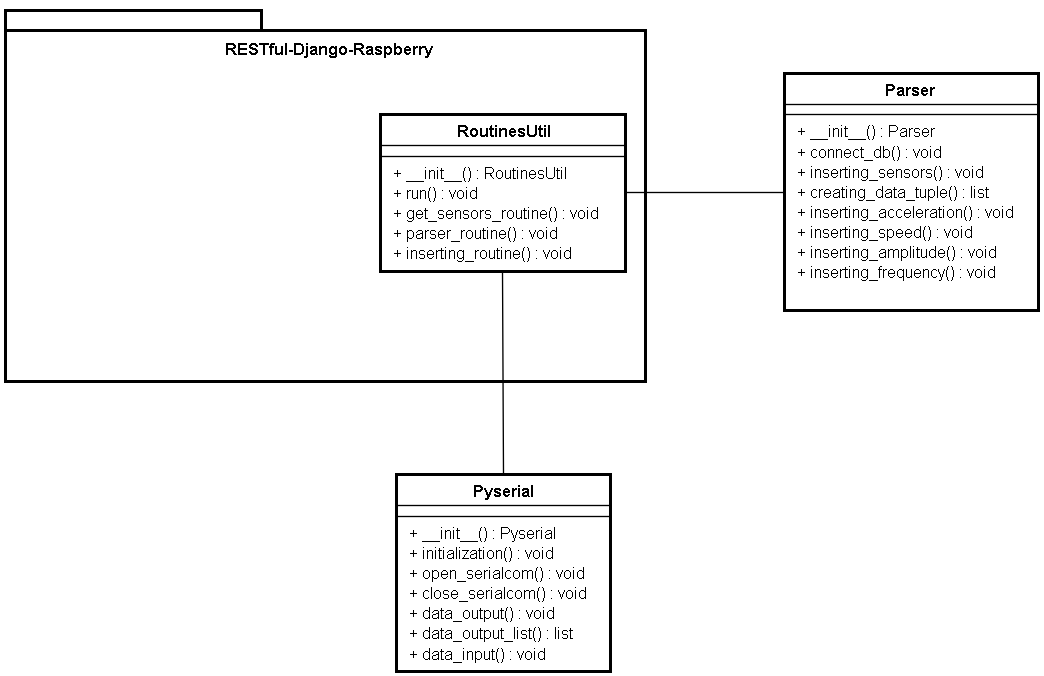
\includegraphics[keepaspectratio=true,scale=0.65]{figuras/uml_routines_parser.png}
\label{fig:uml_routines_parser}
\caption{Diagrama de Classes Parcial das Rotinas de Comunicação e Parser, integrados ao \textit{Django} - Fonte: Autor}
\end{figure}

\subsubsection*{\textbf{Processamento dos Dados}}

A integral é uma das mais importantes ferramentas matemáticas e que aparece com frequência na solução de problemas e no cálculo de grandezas 
na engenharia e na ciência \cite{metodos_numericos}.

Na engenharia, há situações que envolvem dados experimentais ou de teste, nos quais uma grandeza física a ser determinada pode ser expressa 
como a integral de outras grandezas medidas. Assim, é válido ressaltar que o integrando pode ser uma função analítica ou um conjunto de pontos
discretos (dados tabulados).

Quando se tem um integrando expresso de forma que a integral pode ser facilmente calculada, pode-se obter analiticamente o valor da integral 
definida. A integração numérica faz-se necessária quando a integração analítica é difícil, ou mesmo impossível, e quando o integrando é fornecido
como um conjunto discreto de pontos \cite{metodos_numericos}.

Este é o caso da Bancada de Vibrações Mecânicas que está sendo construída neste projeto. Os dados que se tem são o retorno da leitura dos sensores 
e assim, o integrando é fornecido como um conjunto de pontos.

A análise numérica de uma integral caracteriza-se por estimar  o número correspondente à integral de uma função entre os limites [a, b]. 
Caso seja utilizado apenas os pontos finais do intervalo, pode ser que o resultado fornecido não seja suficientemente preciso, especialmente se
o intervalo for significativamente grande ou se o integrando variar significativamente ao longo do intervalo. Dessa maneira, uma maior precisão 
pode ser obtida com o uso de um método composto, no qual o intervalo [a, b] é dividido em subintervalos menores. Assim, calcula-se a integral ao
longo de cada subintervalo e os resultados são somados para fornecer a integral completa.

É importante ressaltar que existem vários métodos disponíveis para o cálculo numérico de integrais. Esses métodos podem ser divididos em abertos 
e fechados. Os métodos de integração fechados consideram os pontos finais do intervalo e o integrando propriamente dito na fórmula que estima o
valor da integral. Já nos métodos de integração abertos, o intervalo de integração se estende além do limite especificado pelos pontos finais 
\cite{metodos_numericos}.

Devido à variedade de métodos, os principais foram analisados e verificou-se sua aplicação no âmbito do projeto. Os métodos considerados foram: 
Trapezoidal Composto, Métodos de Simpson e Quadratura de Gauss.

No {\textbf{Método Trapezoidal Composto}} a integral, ao longo do intervalo [a, b], pode ser avaliada de forma mais precisa com a subdivisão do 
intervalo, a avaliação da integral em cada um dos subintervalos e a soma dos resultados. A imagem a seguir ilustra a expansão genérica para a 
integração numérica por trapézios.

\begin{figure}[H]
\centering
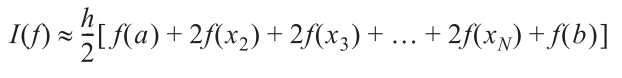
\includegraphics[keepaspectratio=true,scale=0.52]	{figuras/metodo_trapezoidal.png}
\label{fig:metodo_trapezoidal}
\caption{Integração numérica por Trapézios Acumulados - Fonte: \citeonline{metodos_numericos}}
\end{figure}

É importante notar que a fórmula do método trapezoidal composto se aplica precisamente para os casos onde os subintervalos têm uma largura h
idêntica. Outro aspecto interessante no uso desse método é que a precisão da resposta pode melhorar a partir da utilização de mais subintervalos.

O método trapezoidal aproxima o integrando por uma linha reta. De fato, seria melhor a aproximação por meio da representação do integrando 
como uma função não-linear e de fácil integração.

Há um grupo de métodos dotados desta característica, denominados \textbf{Métodos de Simpson}, utilizando polinômios quadráticos (método de
Simpson 1/3) e polinômios cúbicos, no caso do método de Simpson 3/8.

Os métodos de Simpson possuem restrições mais severas para uso. No caso do método de Simpson 1/3 composto, os subintervalos devem ser 
igualmente espaçados e o número de subintervalos no intervalo [a, b] deve ser um número necessariamente par. Com relação ao método de Simpson 
3/8 composto, além do espaçamento igual na identificação dos subintervalos, tem-se que o número de subintervalos no intervalo [a, b] deve ser 
divisível por 3.

Por fim, na \textbf{Quadratura de Gauss}, a integral também é avaliada utilizando a soma ponderada dos valores da função em pontos distintos 
ao longo do intervalo [a, b]. Nessa abordagem, são utilizados os pontos de Gauss, que, por sua vez, não são igualmente espaçados e não incluem 
os pontos finais.

Para o projeto da Bancada de Vibrações, optou-se pelo uso do método dos trapézios acumulados (método trapezoidal composto). A frente de 
controle projetou uma leitura dos dados dos sensores que garantirá intervalos de tempo igualmente espaçados, já favorecendo a aplicação de 
tal método. Outro aspecto interessante é que não será necessário controlar se o número de subintervalos é par ou se é divisível por três. 
O método dos trapézios se aplica independentemente deste aspecto.

Outro aspecto que deve ser notado é que como a massa de dados coletada a partir da leitura das medições feitas pelos sensores é grande, a
precisão do método será ainda maior.